%%%%%%%%%%%%%%%%%%%%%%%%%%%%%%%%%%%%%%%%%
% NIWeek 2014 Poster by T. Reveyrand
% www.microwave.fr
% http://www.microwave.fr/LaTeX.html
% ---------------------------------------
% 
% Original template created by:
% Brian Amberg (baposter@brian-amberg.de)
%
% This template has been downloaded from:
% http://www.LaTeXTemplates.com
%
% License:
% CC BY-NC-SA 3.0 (http://creativecommons.org/licenses/by-nc-sa/3.0/)
%
%%%%%%%%%%%%%%%%%%%%%%%%%%%%%%%%%%%%%%%%%

%----------------------------------------------------------------------------------------
%	PACKAGES AND OTHER DOCUMENT CONFIGURATIONS
%----------------------------------------------------------------------------------------

\documentclass[a0paper,portrait]{baposter}

\usepackage[font=small,labelfont=bf]{caption} % Required for specifying captions to tables and figures
\usepackage{booktabs} % Horizontal rules in tables
\usepackage{relsize} % Used for making text smaller in some places

\usepackage{amsmath,amsfonts,amssymb,amsthm} % Math packages
\usepackage{eqparbox}

\usepackage{textcomp}

\usepackage{hyperref}

\graphicspath{{images/}} % Directory in which figures are stored

 \definecolor{bordercol}{RGB}{40,40,40} % Border color of content boxes
 \definecolor{headercol1}{RGB}{186,215,230} % Background color for the header in the content boxes (left side)
 \definecolor{headercol2}{RGB}{120,120,120} % Background color for the header in the content boxes (right side)
 \definecolor{headerfontcol}{RGB}{0,0,0} % Text color for the header text in the content boxes
 \definecolor{boxcolor}{RGB}{210,235,250} % Background color for the content in the content boxes
 
\definecolor{jdhblue}{RGB}{2,93,186}

\definecolor{zkblue}{RGB}{88,135,175}
\definecolor{zkbackground}{RGB}{230,232,234}


\usetikzlibrary{shapes,arrows,external,decorations.pathmorphing,backgrounds,positioning,fit,petri,calc,hobby,cd}


\begin{document}

% \background{ % Set the background to an image (background.pdf)
% \begin{tikzpicture}[remember picture,overlay]
% \draw (current page.north west)+(-2em,2em) node[anchor=north west]
% {\includegraphics[height=1.1\textheight]{images/baposter_background.pdf}};
% \end{tikzpicture}
% }

\begin{poster}{
grid=false,
borderColor=bordercol, % Border color of content boxes
headerColorOne=headercol1, % Background color for the header in the content boxes (left side)
headerColorTwo=headercol2, % Background color for the header in the content boxes (right side)
headerFontColor=headerfontcol, % Text color for the header text in the content boxes
% boxColorOne=boxcolor, % Background color for the content in the content boxes
boxColorOne=zkbackground,
headershape=roundedright, % Specify the rounded corner in the content box headers
headerfont=\Large\sf\bf, % Font modifiers for the text in the content box headers
textborder=rectangle,
% background=user,
background=none,
headerborder=open, % Change to closed for a line under the content box headers
boxshade=plain
}
%
%----------------------------------------------------------------------------------------
%	TITLE AND AUTHOR NAME
%----------------------------------------------------------------------------------------
%
{
\includegraphics[scale=0.090]{logo_buaa_math.jpg}} % University/lab logo
{
% \bf \LARGE{Hybrid Arrhythmia Detection on Varying-Dimensional ECG} \\
{\bf \fontsize{19pt}{19pt} \selectfont Searching for Effective Neural Network Architectures} \\
{\it \LARGE  for Heart Murmur Detection from Phonocardiogram}
} % Poster title
{\vspace{0.3em} \smaller Hao WEN$^1$, Jingsu KANG$^2$  \\  % Author names
  
$^1${\it LIMB and School of Mathematical Sciences, Beihang University} \\
$^2${\it Tianjin Medical University} \\
\vspace{0.2cm}
{\Large \bf{The George B. Moody PhysioNet Challenge 2022}, ~~~\bf{Team Revenger}}
}
{
\includegraphics[scale=0.103]{logo_tmu.jpeg}}


%----------------------------------------------------------------------------------------
%	INTRODUCTION
%----------------------------------------------------------------------------------------

\headerbox{Introduction}{name=introduction, column=0, row=0, span=3}{
% finished

\begin{itemize}
    \item We used \textbf{neural network models} to make per-recording predictions, then used a simple \textbf{greedy rule} to obtain per-patient predictions.
    \vspace{-0.2cm}
    \item We applied the \textbf{multi-task learning (MTL)} paradigm via hard parameter sharing to make predictions using \textbf{ONE} model. The model has 2 classification heads (murmur and outcome, denoted ``MTL2'') or 3 (denoted ``MTL3'') with an additional segmentation head.
    \vspace{-0.2cm}
    \item We performed extensive \textbf{architecture searching for the backbone (the shared parameters)} of the neural network model.
\end{itemize}
}


%----------------------------------------------------------------------------------------
%	NN architecture
%----------------------------------------------------------------------------------------

\headerbox{Neural Network Backbones}{name=nn, column=0, below=introduction}{
% finished

\includegraphics[width=\linewidth]{images/compare_nn.pdf}

A part of the backbones (the shared representation) we experimented with.

}

%----------------------------------------------------------------------------------------
%	MTL
%----------------------------------------------------------------------------------------

\headerbox{Multi-Task Learning}{name=mtl, span=2, column=1, row=1, below=introduction}{
% finished

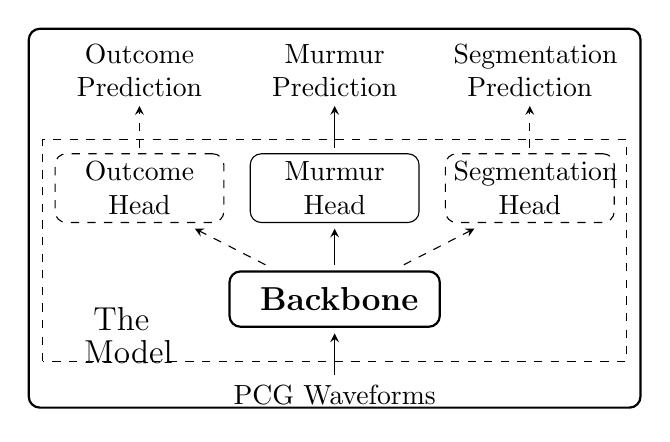
\begin{tikzpicture}

\tikzstyle{block} = [rectangle, draw, text width = 5.5em, text centered, rounded corners, inner sep = 3pt, minimum height = 1.0em]
\tikzstyle{bigblock} = [rectangle, draw, text width = 7em, text centered, rounded corners, thick, inner sep = 3pt, minimum height = 2.0em]

\node (input) {PCG Waveforms};
\node [bigblock, above = 0.6 of input] (backbone) {\textbf{{\larger[1] Backbone}}};
\node [block, dashed, above left = 0.6 and 0.05 of backbone] (outcome) {Outcome Head};
\node [block, above = 0.6 and of backbone] (murmur) {Murmur Head};
\node [block, dashed, above right = 0.6 and 0.05 of backbone] (seg) {Segmentation Head};
\node [text width = 5.5em, text centered, above = 0.6 of outcome] (outcome_pred) {Outcome Prediction};
\node [text width = 5.5em, text centered, above = 0.6 of murmur] (murmur_pred) {Murmur Prediction};
\node [text width = 5.5em, text centered, above = 0.6 of seg] (seg_pred) {Segmentation Prediction};

\path[-stealth] (input) edge ([yshift = -2]backbone.south);
\path[-stealth, dashed] ([xshift = -25, yshift = 2]backbone.north) edge ([xshift = 20, yshift = -2]outcome.south);
\path[-stealth, dashed] ([xshift = 25, yshift = 2]backbone.north) edge ([xshift = -20, yshift = -2]seg.south);
\path[-stealth] ([yshift = 2]backbone.north) edge ([yshift = -2]murmur.south);
\path[-stealth, dashed] ([yshift = 2]outcome.north) edge (outcome_pred.south);
\path[-stealth, dashed] ([yshift = 2]seg.north) edge (seg_pred.south);
\path[-stealth] ([yshift = 2]murmur.north) edge (murmur_pred.south);

\draw[dashed] ([xshift = -35, yshift = -50]outcome.south) rectangle ([xshift = 35, yshift = 5]seg.north);
\node[below = 0.95 of outcome, text width = 4em, align = left] {{\larger[1] The Model}};
\draw[rounded corners, thick] ([xshift = -40, yshift = -109]outcome_pred.south) rectangle ([xshift = 40, yshift = 2]seg_pred.north);

\end{tikzpicture}%
\includegraphics[width=0.5\linewidth]{images/tresnets-clf-vs-mtl.pdf}

The multi-task learning (MTL) paradigm. Experiments indicates its efficacy.

}

%----------------------------------------------------------------------------------------
%	Loss functions comparison
%----------------------------------------------------------------------------------------

\headerbox{Loss Function Choices}{name=loss, column=0, span=1, below=nn}{
% finished

\includegraphics[width=\linewidth]{images/mtl-se-resnet-lossA-vs-lossB.pdf}
% \vspace{-0.5cm}
\begin{itemize}
    \item Loss-A: Asymmetric Loss
    \vspace{-0.2cm}
    \item Loss-B: Weighted BCE Loss
\end{itemize}

}
%----------------------------------------------------------------------------------------
%	Loss functions comparison
%----------------------------------------------------------------------------------------

\headerbox{Demographic Features}{name=dem, column=0, span=1, below=loss}{
% finished

\begin{itemize}
    \item Some demographic features are strongly correlated with ``Outcome''.
    \vspace{-0.2cm}
    \item A random forest classifier using demographic features and the murmur predictions as input improved outcome sores (reduced the outcome cost).
    \vspace{-0.2cm}
    \item Our final submission \textbf{DID NOT} use demographic features and related auxiliary (e.g. random forest) classifiers.
\end{itemize}

}

%----------------------------------------------------------------------------------------
%	Preprocessing, Augmentations
%----------------------------------------------------------------------------------------

\headerbox{Preprocess Pipeline and Augmentations}{name=data, column=1, row=1, span=2, below=mtl}{
% finished
\begin{itemize}
    \item Resampling to 1000 Hz.
    \vspace{-0.2cm}
    \item Butterworth bandpass filtering of order 3 and cutoff frequencies 25 - 400 Hz.
    \vspace{-0.2cm}
    \item Z-score normalization to zero mean and unit variance.
    \item Adding coloured noises.
    \vspace{-0.2cm}
    \item Polarity inversion (flipping).
\end{itemize}
}

%----------------------------------------------------------------------------------------
%	Training Setups
%----------------------------------------------------------------------------------------

\headerbox{Training Setups}{name=training,span=2,column=1,row=1, below=data}{
% finished
\begin{itemize}
    \item Optimizer: AMSGrad variant of {\bf AdamW} with {\bf OneCycleLR} scheduler.
    \vspace{-0.2cm}
    \item Stratified train-validation split: 80\% -- 20\%.
    \vspace{-0.2cm}
    \item Batch size 32; epoch number $\leq 60$ with early stopping.
    \vspace{-0.2cm}
    \item Freeze backbone from specific epoch (typically 30).
\end{itemize}
}


%----------------------------------------------------------------------------------------
%	Submission Results
%----------------------------------------------------------------------------------------

\headerbox{Submission Results}{name=submission, span=2, column=1, below=training}{
% finished
\begin{center}
\begin{tabular}{r|c|c|c}
    \hline
    & \textbf{Murmur} & \multicolumn{2}{c}{\textbf{Outcome}} \\
    & \textbf{weighted accuracy} & \multicolumn{1}{c}{\textbf{cost}} & \multicolumn{1}{c}{weighted accuracy} \\ \hline
    Train & $0.88\pm 0.05$ & $8452\pm 2324$ & $0.88\pm 0.07$ \\
    Train-val & $0.86\pm 0.01$ & $11341\pm 336$ & $0.79\pm 0.05$ \\ \hline
    Hidden val & \textbf{0.689} & \textbf{9471.652} & NA \\
    Ranking & \textbf{79/303} & \textbf{21/303} & NA \\ \hline
\end{tabular}
\end{center}
Scores on the train, and train-val sets are provided with mean and standard deviation over most of our offline experiments. Scores on the hidden validation set are provided with the best scores out of the 10 submissions.
}

%----------------------------------------------------------------------------------------
%	Limitations, Discussions
%----------------------------------------------------------------------------------------

\headerbox{Discussions and Limitations}{name=discussion, column=0, below=dem, span=3}{
% not finished
\begin{itemize}
\item Our multi-task learning (MTL) paradigm proved practical for the problems of heart murmur detection and clinical outcome identification from PCGs. The additional segmentation head makes the shared representation (the common backbone) learn more general features and thus improves the performances for the original two classification tasks the Challenge raised.
\vspace{-0.2cm}
\item All our models used \textbf{time-domain} signals, i.e. the \textbf{waveforms} as inputs. The derived \textbf{time-frequency-domain} signals, for example, the \textbf{spectrograms}, were not tested. Models that accept mixed-type inputs were not tested either.
\vspace{-0.2cm}
\item The need for Z-score normalization has to be reconsidered. More frequency-domain augmentation methods should be applied.
\vspace{-0.2cm}
\item The convolutional neural backbones proved effective, but still have room for improvements compared to top teams.
\vspace{-0.2cm}
\item The potential of models with the \textbf{transformer architecture} (e.g. the \textbf{wav2vec2} model) were not fully explored. As well as the powerfulness of model pretraining via self-supervised learning on larger datasets (e.g. the PhysioNet EPHNOGRAM dataset, etc.).
\end{itemize}
}


%----------------------------------------------------------------------------------------
%	REFERENCES
%----------------------------------------------------------------------------------------

%\headerbox{References}{name=references,column=2,below=application}{

%\smaller % Reduce the font size in this block
%\renewcommand{\section}[2]{\vskip 0.05em} % Get rid of the default "References" section title
%\nocite{*} % Insert publications even if they are not cited in the poster

%\bibliographystyle{unsrt}
%\bibliographystyle{IEEEtran}
%\bibliography{biblio} % Use biblio.bib as the bibliography file
%}


%----------------------------------------------------------------------------------------
%	ACKNOWLEDGEMENTS
%----------------------------------------------------------------------------------------

\headerbox{Acknowledgements}{name=acknowledgements, column=0, below=discussion, span=3}{
% finished
% \smaller
We would like to thank professor {\bf Deren Han} from the School of Mathematical Sciences, Beihang University and professor {\bf Wenjian Yu} from the Department of Computer Science and Technology, BNRist, Tsinghua University for generously providing GPU servers to help accomplish this work.

% \hfill \small \textit{Code, configs, etc. available at \href{https://github.com/DeepPSP/cinc2021}{https://github.com/DeepPSP/cinc2021}.}
}

%----------------------------------------------------------------------------------------
%	link to the github repository
%----------------------------------------------------------------------------------------

\headerbox{}{name=foottext, column=0, span=3, below=acknowledgements, textborder=none, headerborder=none,  boxheaderheight=0pt}{
% finished
\hfill \small \textit{Code, configs, etc. available at https://github.com/DeepPSP/cinc2022}.
}


\end{poster}

\end{document}
